\chapter{Comparch II - Part 4a. Instruction Level Parallelism Performance}
\textit{So far, we've only been building our processor, now it's about performance\dots}
\section{What is Performance ?}
\textit{Now what do we mean by performance ?, we need a metric to measure performance.}
\begin{itemize}
    \item[] Does processory frequency matter ? \textit{Is it better an Intel Core i7-7700K at 4.2 GHz or an AMD Ryzen 5 5600X at 3.7 GHz?}
    \item[] Memory Speed ? Cache efficiency ?
    \begin{itemize}
        \item[] Is it better to have 8 MiB of 4-way set-associative cache or 16 MiB of direct
        mapped cache?
        \item[] Is it better to have three levels of overall smaller caches or two levels of overall
        bigger caches?
    \end{itemize}
\end{itemize}
\subsection{Elapsed Time, CPU Time, \dots}
\textit{In reality, none of this matters in it self.}
What matters is the time it takes to perform a job a user needs.
\begin{center}
    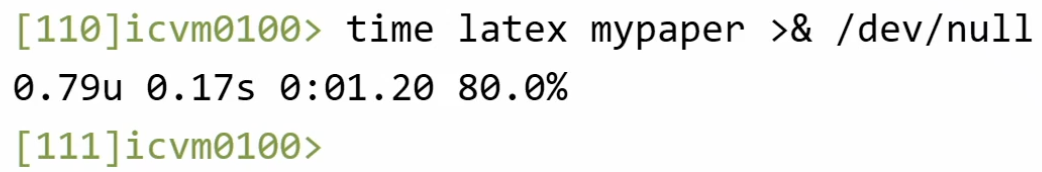
\includegraphics[width=0.45\textwidth]{chapters/chapter4a/images/elapsed.png}
\end{center}

\begin{itemize}
    \item \textbf{Elapsed Time:} The total time taken for the job to complete, measured from start to finish. (e.g., 1.20 seconds)
    \item \textbf{System CPU Time:} The CPU time used by the operating system to execute instructions on behalf of the program. (e.g., 0.17 seconds)
    \item \textbf{User CPU Time:} The CPU time used to execute instructions for the program itself. (e.g., 0.79 seconds)
    \item 80.0\% of the Elapsed Time ($0.96\,s / 1.20\,s$) was spent on the job (the rest might be spent on system I/O, other jobs, and other users.)
    \item \textbf{Note:} \textit{User CPU Time} + \textit{System CPU Time} $\neq$ \textit{Elapsed Time}: The processor spent 0.96 seconds executing for the program, but the overall job took 1.20 seconds to complete.
\end{itemize}

\subsection{Relative Performance}
\textbf{Speedup}

The speedup metric quantifies how much faster system $X$ is compared to system $Y$. It is defined as:
\[
\text{Speedup} = \frac{\text{Performance}_X}{\text{Performance}_Y} = \frac{\text{Execution Time}_Y}{\text{Execution Time}_X}
\]

\textbf{Common Performance Indices}
Common benchmarks used to measure the speedups of systems relative to a standard system include: \newline
\textbf{SPEC CPU} (a classic CPU performance benchmark), \textbf{Geekbench} (a comprehensive cross-platform benchmark), \textbf{Cinebench} (a benchmark focusing on rendering performance), \textbf{LinPack HPL} (a high-performance computing benchmark), and \textbf{EEMBC (``Embassy'') CoreMark} (dedicated to benchmarking embedded processors).

\subsection{Relating Performance to Hardware Implementation}
In hardware design, time is measured by the \textit{clock period} or \textit{cycle}.

\subsubsection{Cycles per Instruction (CPI) and Instructions per Cycle (IPC)}
\begin{itemize}
    \item CPI: Average cycles needed per instruction
    \[
    \text{CPI} = \frac{\text{Total Cycles}}{\text{Total Instructions}} = \frac{\text{Execution Time}/\text{Clock Period}}{\text{Total Instructions}}
    \]
    \item IPC: Average instructions executed per cycle
    \[
    \text{IPC} = \frac{1}{\text{CPI}}
    \]
    \item Note: IPC $\leq$ 1 unless the processor can execute multiple instructions in parallel
\end{itemize}

\subsection{Improving Performance}
Performance is defined as the reciprocal of execution time:

\[
\text{Performance} = \frac{1}{\text{Execution Time}}
\]

By breaking down execution time, performance can be expressed as:

\[
\text{Performance} = \frac{f_{\text{clock}}}{\text{Instruction Count} \cdot \text{CPI}} = \frac{f_{\text{clock}}\cdot IPC}{\text{Instruction Count}}
\]

Where:
\begin{itemize}
    \item[] $f_{\text{clock}}$ is the clock frequency.
    \item[] $\text{CPI}$ is the cycles per instruction.
    \item[] $\text{Instruction Count}$ is the total number of instructions executed.
\end{itemize}

To improve performance, several strategies can be employed:

\begin{enumerate}
    \item \textbf{Increase Clock Frequency ($f_{\text{clock}}$):} Implement the processor using faster technology to achieve higher clock rates.
    \item \textbf{Reduce CPI:} Simplify instructions (RISC architecture) to lower the cycles per instruction. However, this may require more instructions to perform the same task.
    \item \textbf{Decrease Instruction Count:} Use fewer, more complex instructions (CISC architecture). This could increase the number of cycles per instruction or reduce the clock frequency.
    \item \textbf{Execute Instructions in Parallel:} Increase instructions per cycle (IPC) through techniques like pipelining or parallel execution.
\end{enumerate}
These trade-offs highlight the balance required when optimizing computer architecture for performance.

\subsection{Factors Influencing Performance}
Several factors can significantly impact system performance. Here are a few examples:

\begin{itemize}
    \item \textbf{Instruction Count and the Compiler:}
    \begin{itemize}
        \item The instruction count depends heavily on the compiler.
        \item A well-designed instruction set that the compiler can use effectively (i.e., best instructions for the job) is more important than having a highly reduced or overly complex instruction set. Otherwise, the instruction count may become unnecessarily large.
    \end{itemize}

    \item \textbf{Cycles Per Instruction (CPI) and Cache Performance:}
    \begin{itemize}
        \item CPI is influenced by the efficiency of the cache.
        \item As the overall code size increases, cache performance may degrade due to a higher number of cache misses.
    \end{itemize}

    \item \textbf{Clock Cycle Speed and Memory Access:}
    \begin{itemize}
        \item Faster clock cycles increase the demand for fetching instructions from memory.
        \item As a result, the performance of the cache becomes more critical in maintaining overall efficiency.
    \end{itemize}
\end{itemize}

\subsection{What to Improve to Increase Performance}

\textbf{Amdahl's Law (Law of Diminishing Returns)}:
The performance enhancement possible with a given improvement is limited by the amount the improved feature is used. \\

\textbf{Typical Software Situation:} \\
If a program spends 20\% of its time in subroutine $X$, the maximum reduction in execution time achievable by optimizing $X$ is 20\%. This corresponds to a speedup of:
\[
\text{Speedup} = \frac{1}{1 - 0.2} = 1.25
\]

\textbf{In a Processor:} \\
If an instruction $Y$ is used only 0.1\% of the time, is it worth optimizing it? It is more practical to focus on optimizing instructions or operations used more frequently, such as those taking 20\% of the time.

What often happens is that we start optimizing the most used instructions, but then we forget that once optimized, the less used instructions become the bottleneck. So, we need to start looking at the less used instructions and optimize them, and so on.
\begin{center}
\textbf{\textcolor{red}{Look for where most of the time goes!}}
\end{center}

\subsection{Benchmarks}

\textbf{Performance Indices:} \\
Benchmarks such as SPEC CPU, Geekbench, Cinebench, LinPack HPL, and EEMBC ("Embassy") CoreMark require a \textbf{precise definition of the user job(s)} to be executed. \\

\textbf{Benchmark Suites:} \\
Serious \textbf{benchmark suites} consist of collections of large and representative user programs, spanning various areas of typical use. These suites are often agreed upon by manufacturers to ensure standardization. \\

\textbf{Key Features:} \\
Benchmark suites do not only define the programs (e.g., written in C, C++, FORTRAN, or Java), but also specify: \\
\begin{itemize}
    \item How the programs should be compiled.
    \item What data should be used during execution.
    \item The conditions under which the programs should be run.
\end{itemize}

\subsubsection{SPEC CPU2006 Integer Benchmarks}
The SPEC CPU2006 benchmark suite evaluates the performance of computer processors by running a set of standardized workloads. Below is a comparison of integer benchmarks between SPEC CPU2000 and SPEC CPU2006. The benchmarks are categorized by their description, language, and reference time (RT).


\begin{center}
    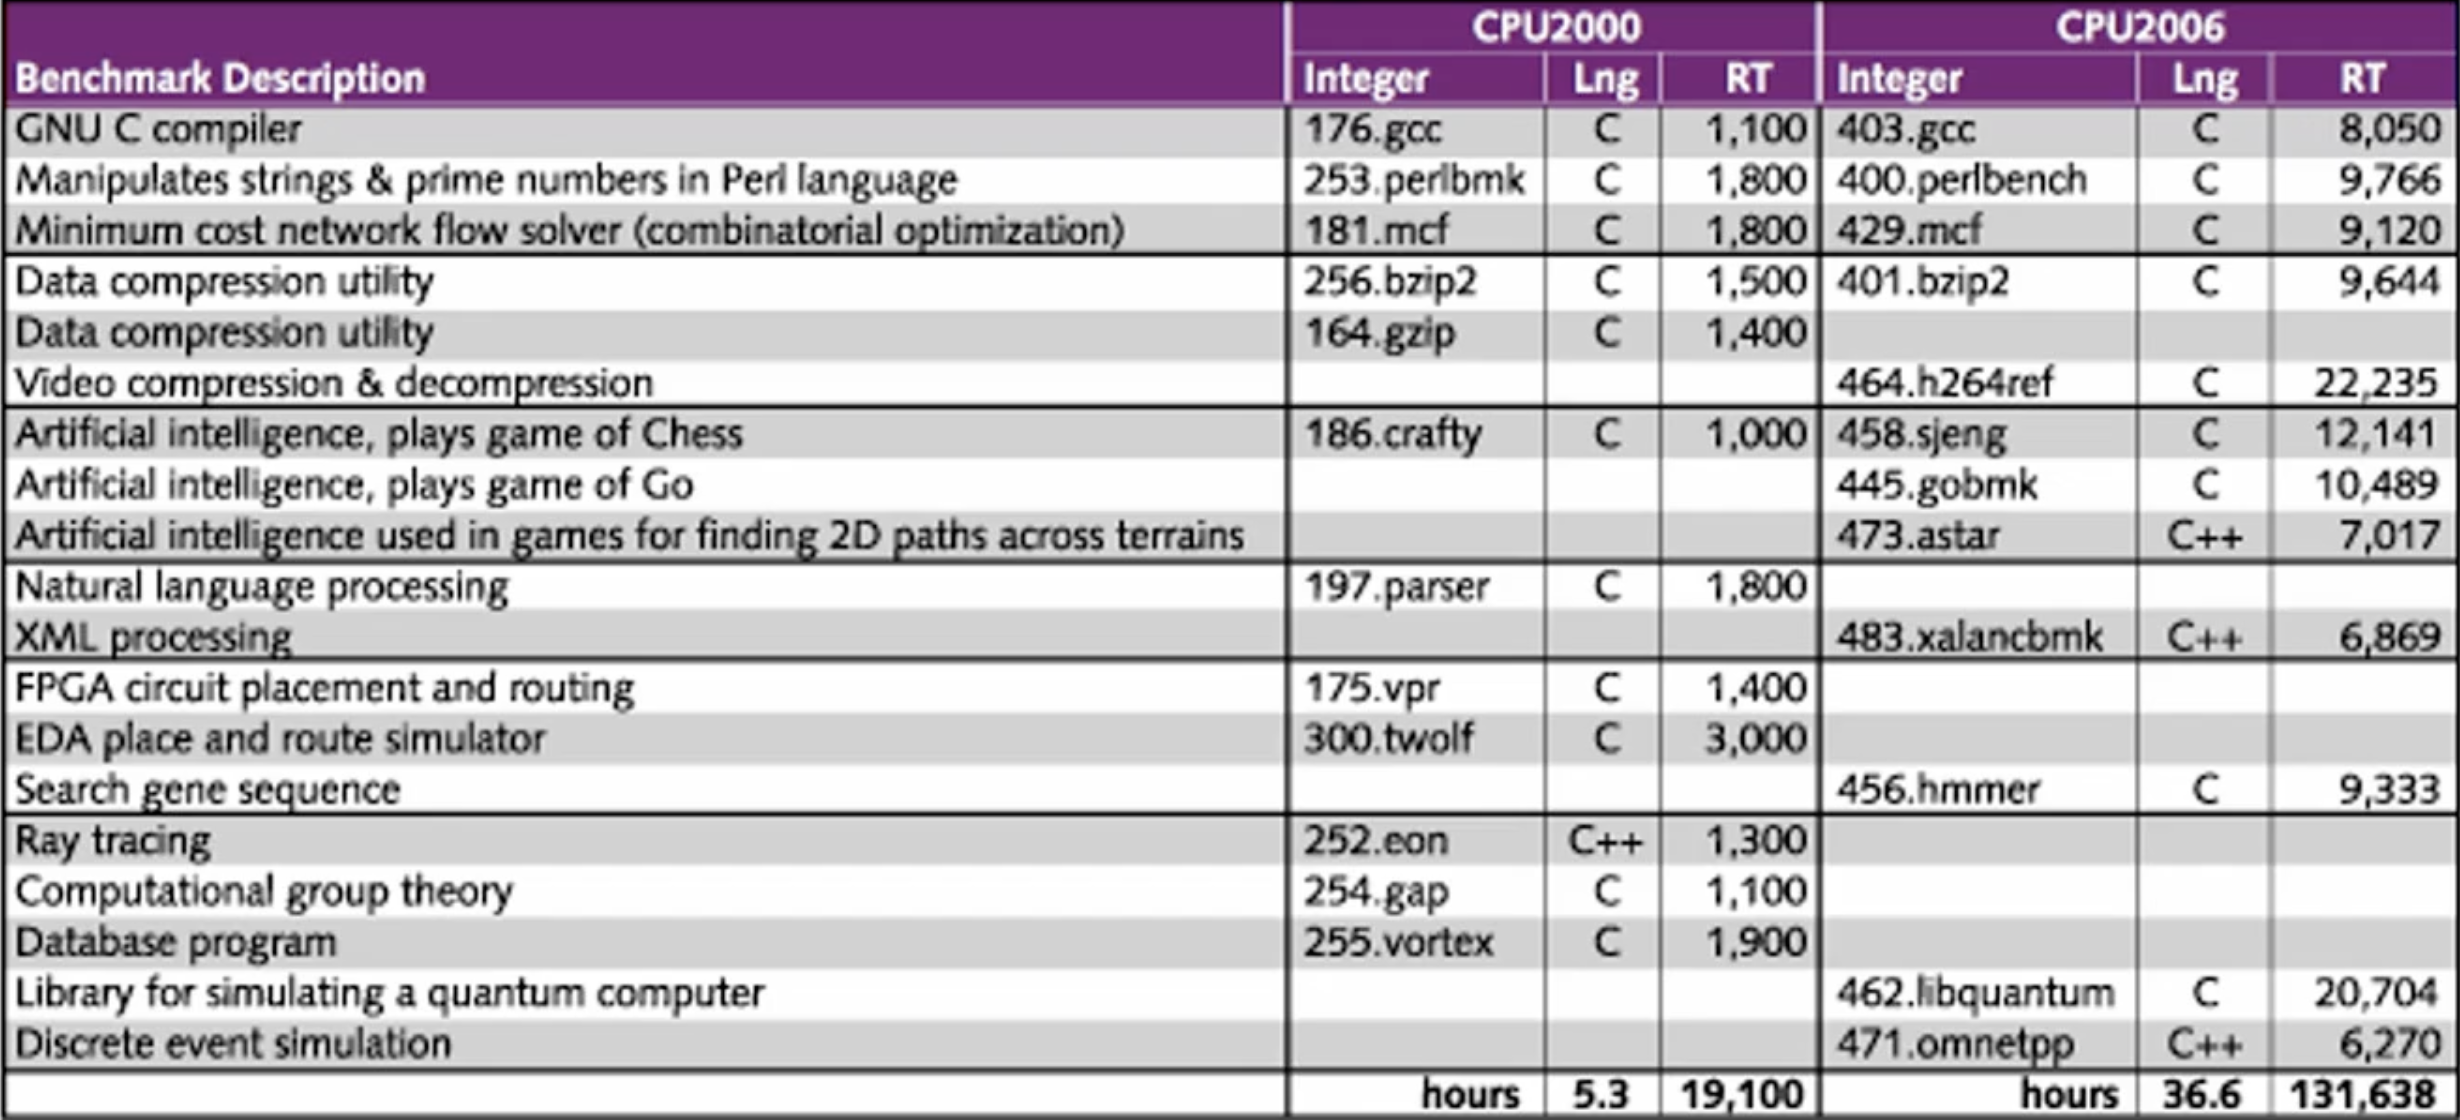
\includegraphics[width=0.65\textwidth]{chapters/chapter4a/images/spec.png}
\end{center}

\textbf{Key Notes:}
\begin{itemize}
    \item \textbf{Reference Time (RT):} Measured on a Sun Ultra 5 with a 300MHz UltraSPARC III and 256KB L2 cache, corresponding to 100 SPEC2000.
    \item \textbf{Benchmark Complexity:} The runtime for integer benchmarks was 36.6 hours on a relatively old machine.
    \item SPEC CPU2006 introduced more complex workloads and higher reference times, demonstrating a significant evolution in benchmarking standards.
\end{itemize}
